%%%%%%%%%%%%%%%%%%%%%%%%%%%%%%%%%%%%%%%%%%%%%%%%%%%%%%%%%%%%%%%%%%%%%%%%%%%%%%%%
%2345678901234567890123456789012345678901234567890123456789012345678901234567890
%        1         2         3         4         5         6         7         8

\documentclass[letterpaper, 10 pt, conference]{ieeeconf}  % Comment this line out
                                                          % if you need a4paper
%\documentclass[a4paper, 10pt, conference]{ieeeconf}      % Use this line for a4
                                                          % paper

\IEEEoverridecommandlockouts                              % This command is only
                                                          % needed if you want to
                                                          % use the \thanks command
\overrideIEEEmargins
% See the \addtolength command later in the file to balance the column lengths
% on the last page of the document



% The following packages can be found on http:\\www.ctan.org
%\usepackage{graphics} % for pdf, bitmapped graphics files
%\usepackage{epsfig} % for postscript graphics files
%\usepackage{mathptmx} % assumes new font selection scheme installed
%\usepackage{times} % assumes new font selection scheme installed
%\usepackage{amsmath} % assumes amsmath package installed
%\usepackage{amssymb}  % assumes amsmath package installed

\usepackage{graphicx}
\usepackage{hyperref}
\usepackage{listings}
\widowpenalties 1 10000
\raggedbottom

\title{\LARGE \bf
Parallelization of Greedy Algorithms
}

%\author{ \parbox{3 in}{\centering Huibert Kwakernaak*
%         \thanks{*Use the $\backslash$thanks command to put information here}\\
%         Faculty of Electrical Engineering, Mathematics and Computer Science\\
%         University of Twente\\
%         7500 AE Enschede, The Netherlands\\
%         {\tt\small h.kwakernaak@autsubmit.com}}
%         \hspace*{ 0.5 in}
%         \parbox{3 in}{ \centering Pradeep Misra**
%         \thanks{**The footnote marks may be inserted manually}\\
%        Department of Electrical Engineering \\
%         Wright State University\\
%         Dayton, OH 45435, USA\\
%         {\tt\small pmisra@cs.wright.edu}}
%}

\author{Matthew Dowdy, Omar Mosa, Brandon Surh, Ethan Kaplan}


\begin{document}



\maketitle
\thispagestyle{empty}
\pagestyle{empty}


%%%%%%%%%%%%%%%%%%%%%%%%%%%%%%%%%%%%%%%%%%%%%%%%%%%%%%%%%%%%%%%%%%%%%%%%%%%%%%%%
\begin{abstract}

Many areas of work rely on algorithms to solve problems in their given field. With versatile and efficient algorithms, greedy algorithms come to mind. With greedy algorithms being widely used, optimizing them would have a large impact on the technological world. In this paper, we try to optimize a greedy algorithm through parallelization, specifically Djikstra’s algorithm. We compare a normal implementation to a parallelized implementation and see how the two performances differ. This will give us an insight into the kind of results come with parallelizing greedy algorithms. If there is a positive significant change in performance, then parallelization is a viable option to optimize greedy algorithms.

\end{abstract}


%%%%%%%%%%%%%%%%%%%%%%%%%%%%%%%%%%%%%%%%%%%%%%%%%%%%%%%%%%%%%%%%%%%%%%%%%%%%%%%%
\section{INTRODUCTION}

Greedy algorithms are widely used due to their simplicity and efficiency, even if they don’t find the most optimal solution in every scenario. Its application can be seen in areas such as data compression, sequencing, minimum-cost spanning trees of weighted undirected graphs, and networking. [1] Due to their versatility and applicability, greedy algorithms are important for many areas of computer science and would benefit from runtime optimization. 

Because of the speed and usefulness of greedy algorithms, we investigated if the performance of greedy algorithms could be improved through parallelization. There are immediate challenges with this, particularly as many of these algorithms are inherently sequential. To take an example, to find a solution for the fewest number of coins (the coin problem), we must keep track of how much money is not yet represented in coins. There is not an immediately obvious way to divide this kind of work among multiple threads in a way that nets a performance gain, because finding the coin with the highest value is trivial to determine sequentially and would not benefit from parallelism.

\caption{Example of a greedy algorithm finding the fewest number of US coins to represent a given number of cents. This algorithm would not benefit from parallelization.}
\begin{lstlisting}[language=Java]
public static int fewestUSCoins(int cents) 
{
    int[] coins = {25, 10, 5, 1};
    int count = 0;
    for (int coin : coins) {
   	 count += cents / coin;
   	 cents = cents % coin;
    }
    return count;
}
\end{lstlisting}

However, finding the optimal solution at a certain iteration may not be trivial to determine in every case, and in such cases it may be possible to divide this work among multiple threads to improve performance.

This paper will explore various greedy algorithms and the approaches we took to parallelize them. It will also analyze the runtimes of our solutions, and evaluate the benefits and drawbacks of our algorithm designs.

\section{Greedy Algorithms}
Greedy is a category of algorithms that make a sequence of choices where each choice is the best possible option at the given moment. (1) The name greedy comes from selecting the best choice which is done without regards to future possible options. Greedy algorithms make steps forward and are unable to take steps backward. This affects their ability to find optimal solutions in some cases, but generally work as simple and efficient approaches.

These algorithms work off of optimizing its solution at each “greedy” choice it makes. They will always choose the step that benefits them the most at a particular moment. For example, in the knapsack problem, a greedy algorithm will select the largest possible item to fit into the knapsack at each step. These steps are final and do not backtrack which leads the algorithm to sometimes produce locally optimal solutions rather than the best possible solution or the globally optimal solution.

In cases where greedy algorithms don’t yield the most optimal solution, they can be used as heuristics to find locally optimal solutions. This is why greedy algorithms are versatile and can be applied to many different problems. Locally optimal solutions are solutions that are more feasible than the ones in the vicinity and would look like a peak if visualized with a graph (2). In the graphic to the right, the locally optimal solutions are the peaks with yellow at the tip and the globally optimal solution would be the peak with red. Locally optimal solutions are sometimes used as a heuristic for the problem at hand because it is “good enough”. Globally optimal solutions are the best possible solution and if visualized would be the highest point on a graph.

\begin{figure}
\centering
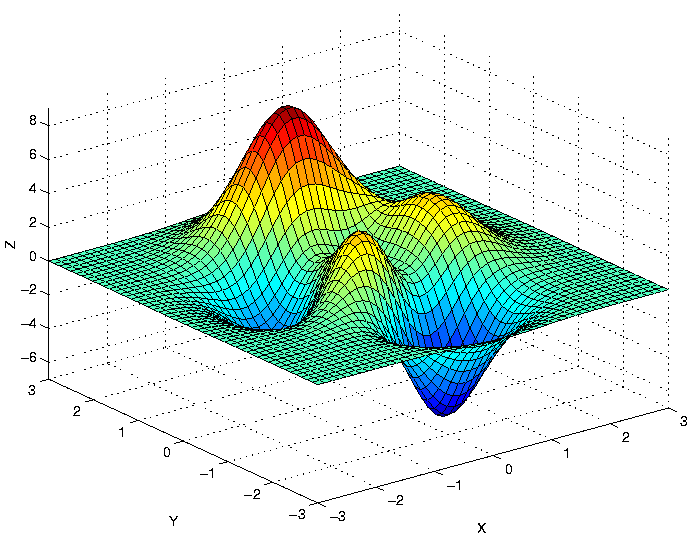
\includegraphics[width=.4\textwidth]{peaks.png}
\caption{Visualization of solutions on a graph.}
\end{figure}

Some common greedy problems include, the knapsack problem, job sequencing problem, graph coloring problem, and the single-source shortest paths problem or Djikstra’s algorithm. In the next section, we will explore Djikstra’s algorithm and its properties to possibly optimize its efficiency.

\section{Dijkstra's Algorithm}

Dijkstra’s algorithm is a greedy algorithm for finding the shortest path between nodes in a graph. In graph theory, this problem has two names: the single source shortest path problem and the all pairs shortest path problem. The single source variant involves finding the shortest path between the source node and the destination node whereas the all-pairs variant involves finding the shortest path between the source node and every other node in the graph. Dijkstra’s algorithm can be modified to solve either of these problems, but we are going to primarily be exploring the all-pairs shortest path problem.

Each implementation of this algorithm uses a Node class with the following data structures:

\begin{lstlisting}[language=Java]
class Node {
    int id;
    Map<Node, Integer> neighbors;
    int distToSource;
    Node prevNode;
}
\end{lstlisting}

The sequential implementation [3] is as follows. Each node is initialized with a distToSource of infinity (except source is initialized to 0) and prevNode of null. Each node is added to the queue. While the queue isn’t empty, the node in the queue which currently has the smallest distToSource is selected as curNode. curNode is removed from the queue. Then, for each neighbor of curNode, add distance from curNode to its neighbor to curNode’s distToSource. If that value is smaller than the neighbor’s distToSource, update the neighbor’s distToSource and mark neighbor’s prevNode as curNode. Repeat until the queue is empty.

\subsection{Naive Parallel Dijkstra}

The parallelization of Dijstra’s algorithm started with a naive solution of simply running each pair of source S and destination D on the single source shortest path (SSSP) algorithm. Then, each thread would take a pair (S, D) and run SSSP. A local copy if the distances and previous nodes are kept on each thread as a map from the node to the distance, and the node to the node, respectively. The code of the SSSP Dijkstra’s algorithm is identical to the APSP, with the exception that after curNode is set, if curNode is the target node, then add the local values of distance and prevNode to the global maps of distance and prevNode and halt the thread. When all threads are halted, the APSP algorithm halts.

This algorithm performs worse than sequential. Figure 2 displays the profiler call tree percentage runtime for the naive parallel algorithm. It shows that HashMap.get() takes 31.9\% of the runtime, HashMap.put\(\) takes 9.6\% of the runtime, and Node.getDistanceToNeighbor() takes up 6.2\% of the runtime (recall that neighbors is a HashMap within the Node class).  

We believe that the runtime of this algorithm is significantly impacted by contention of memory resources. All of the nodes originate from the same set, so each node is only found in memory once. Every node is accessible by every thread, so there are many instances where thread 1 calls HashMap.get(A), where A is an arbitrary Node, but thread 2 has already made an update to A. This causes thread 1 to invalidate its cache line and wait for thread 2 to give thread 1 and main memory the updated value. 

\begin{figure}
\centering
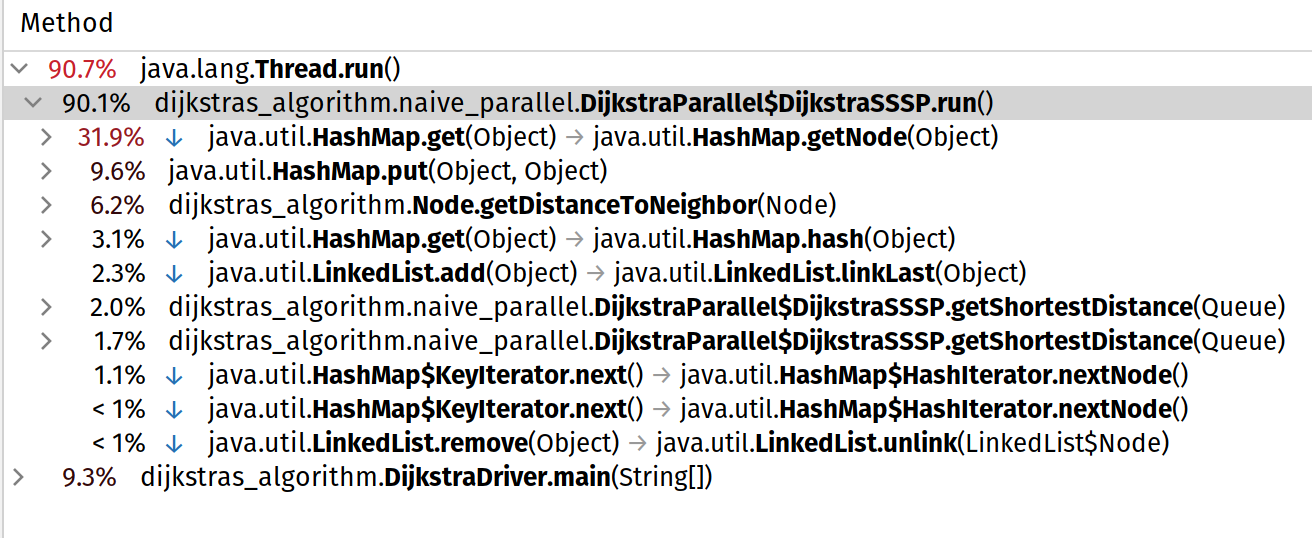
\includegraphics[width=.4\textwidth]{output.png}
\caption{Profiler output from Intellij IDEA Ultimate depicting the runtime of the naive parallel dijkstra's algorithm with a complete graph containing 2000 nodes.}
\end{figure}

Runtime is significantly poor also because of context switching. A thread is spawned for each node in the graph, so when the number of hardware and software threads are about the same, this could be fine, but when the number of software threads greatly outpaces the number of hardware threads, context switching between software threads on hardware becomes a major slowdown. 

\subsection{Parallel Dijkstra using an Authority}

This parallel algorithm splits the nodes set among all threads on the system such that each thread’s subset localNodes is disjoint from every other thread’s localNodes. Each thread maintains a set called cluster and another set called nonCluster [4]. One node is designated the globalAuthority. This node will compare local minimum values to determine what the global minimum distance is [5].

The cluster is initialized with the source node, and nonCluster is initialized with all localNodes that aren’t the source. Then while the nonCluster isn’t empty, each thread finds its node with the least distToSource called localMinNode. Each thread gives its localMinNode to the globalAuthority with the function extractGlobalMin to decide which localMinNode is the globalMinNode. Each thread adds the globalMinNode to its cluster set and removes it from its nonCluster set. 

This version of parallel Dijkstra contains a few more instance variables:

\begin{lstlisting}[basicstyle=\scriptsize, language=Java]
class DijkstraParallel 
{
    ConcurrentSet<Node> decideGlobalMinSet;
    AtomicMarkableReference<Node> globalMinNodeReference;
    AtomicBoolean previousAuthorityToggle;
    AtomicInteger numActiveThreads;
}
\end{lstlisting}

In the function extractGlobalMin, if the thread is not the globalAuthority, it decrements numActiveThreads and busy waits until globalMinNodeReference’s mark changes. Then it returns the reference of globalMinNodeReference.

If the thread is the globalAuthority, it busy waits until numActiveThreads is equal to 1 (the globalAuthority is the only active thread). Then, it iterates over all Nodes in decideGlobalMinSet and finds the Node with the smallest distToSource. It then clears the decideGlobalMinSet, resets numActiveThreads, and sets globalMinNodeReference to the global minimum node with a mark opposite of what it previously was. 

The performance of this version of parallel dijkstra still performs poorly, but it does perform better than the naive solution to parallelize dijkstra’s algorithm. 

\begin{figure}
\centering
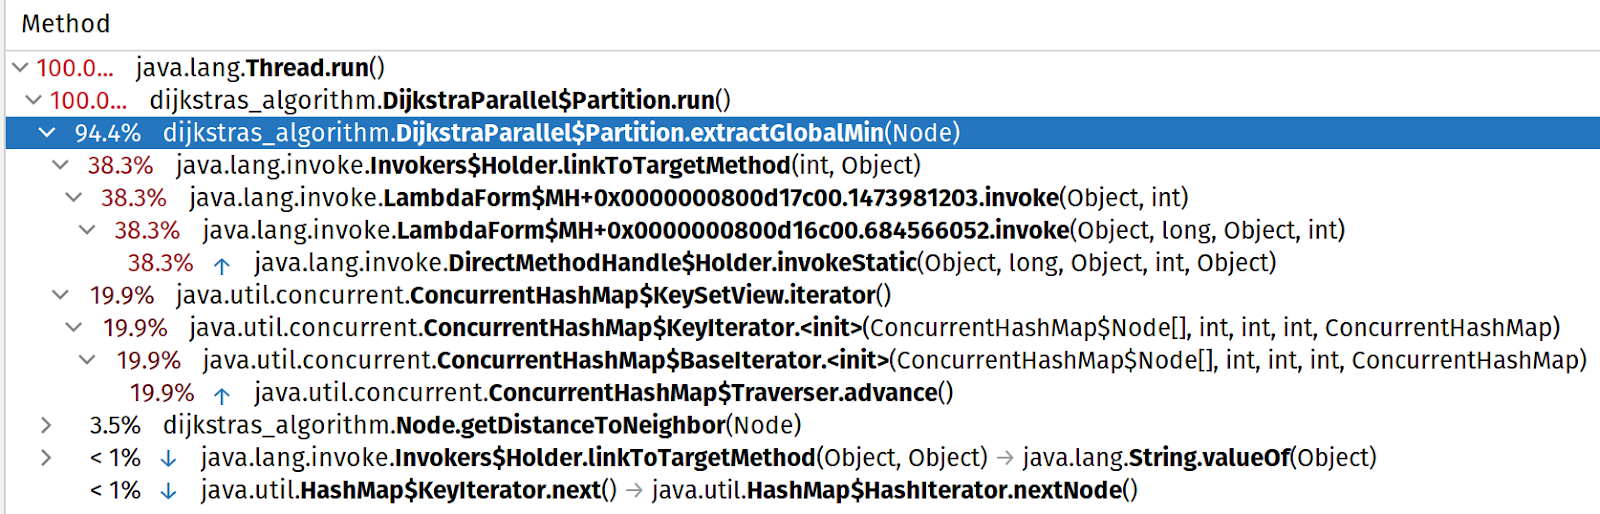
\includegraphics[width=.4\textwidth]{extractGlobalMin.png}
\caption{Profiler output from Intellij IDEA Ultimate of class dijkstras\_algorithm. DijkstraParallel with 2000 node complete graph. Function extractGlobalMin takes 94.4 percent of the runtime.}
\end{figure}

An example of this performance is that with a 2000 node complete graph, the sequential implementation took 0.24 seconds, the naive parallel implementation took 21.13 seconds and this implementation took 1.55 seconds. So this is a significant improvement from the naive approach, but there is still a large room for improvement.

Figure 3 shows the profiler call tree of one thread from this algorithm. Something interesting to note is that 94.4\% of the time is spent in extractGlobalMin. That is when the globalAuthority is waiting for threads to give it their local minimum node and when normal threads (non authority) wait for the authority to make a decision on the global minimum. 
The most significant function within extractGlobalMin(), with 38.3\%, is intelligible internal java code. The next highest runtime occurs in the ConcurrentHashMap iterator. This occurs in the authority’s portion of the code, when it is comparing distToSource values with each local minimum node. 

We believe there is more to improve with this implementation. When the authority releases the updated global minimum node, all threads see that they are ready to resume the program at the same time. This introduces contention on the globalMinNodeReference variable, very similarly to that of the TASLock in the textbook. Therefore, we will implement a queue lock to avoid this unnecessary contention. 

\section{Parallel Processing}



%%%%%%%%%%%%%%%%%%%%%%%%%%%%%%%%%%%%%%%%%%%%%%%%%%%%%%%%%%%%%%%%%%%%%%%%%%%%%%%%



\begin{thebibliography}{99}

 
\bibitem{c1} \href{https://www.solver.com/global-optimization#:~:text=A\%20locally\%20optimal\%20solution\%20is\%20one\%20where\%20there,\%22in\%20the\%20vicinity\%22\%20with\%20better\%20objective\%20function\%20values.}{Global Optimization Methods | solver}
\bibitem{c2} \href{https://en.wikipedia.org/wiki/Dijkstra\%27s_algorithm}{Dijkstra's Algorithm}
\bibitem{c3} \href{https://cse.buffalo.edu/faculty/miller/Courses/CSE633/Ye-Fall-2012-CSE633.pdf}{An Implementation of Parallelizing Dijkstra’s algorithm}
\bibitem{c4} \href{https://citeseerx.ist.psu.edu/viewdoc/download?doi=10.1.1.64.8113&rep=rep1&type=pdf}{ Parallel Algorithms for geometric shortest path problems}
\bibitem{c5} \href{https://core.ac.uk/download/pdf/82042073.pdf}{The classification of greedy algorithms}




\end{thebibliography}


\end{document}
